\documentclass[oneside]{book}

\usepackage[french]{babel}
\usepackage{enumerate}
\usepackage{graphicx}
\usepackage{caption}
\usepackage{subcaption}
\usepackage{geometry}
\usepackage{titlesec}
\usepackage[T1]{fontenc}
\usepackage[dvipsnames]{xcolor}
\usepackage{float}
\usepackage{hyperref}
% \usepackage{fancyhdr}
% \usepackage[Glenn]{fncychap}
\usepackage{biblatex}
\usepackage{csquotes}
\usepackage{wrapfig}
\usepackage[acronym,toc]{glossaries}
\usepackage{xcolor,colortbl}
\usepackage{tikz}
\usepackage{amsmath}
\usepackage{amsfonts}
\usepackage{algorithm}
\usepackage{algpseudocode}
\usepackage{multirow}
\usepackage{lscape}
\usetikzlibrary{positioning}
\addbibresource{extras/references.bib}





\graphicspath{{images/}}
\titleformat{\subsection}[block]{\hspace{3em}}{\thesubsection}{1em}{}
\titleformat{\subsubsection}[block]{\hspace{6em}}{\thesubsection}{1em}{}
\newgeometry{bottom=25mm,left=20mm,top=15mm,right=20mm}
\hypersetup{
    colorlinks,
    citecolor=blue,
    filecolor=blue,
    linkcolor=blue,
    urlcolor=blue
}
\definecolor{Gray}{gray}{0.85}
\pagestyle{headings}
\newcommand*{\captionsource}[2]{%
    \caption[{#1}]{%
    #1%
    \\\hspace{\linewidth}%
    \textbf{Source:} #2%
  }%
}
\setcounter{secnumdepth}{3}
\setcounter{tocdepth}{3}




\makeglossaries
\newacronym{moplazer}{MoPlaZer}{Moroccan Plate RecogniZer}
\newacronym{ia}{IA}{Intelligence Artificielle}
\newacronym{lapi}{LAPI}{Lecture Automatisée de Plaques d'Immatriculation}
\newacronym{anpr}{ANPR}{Automatic Number Plate Recognition}
\newacronym{ocr}{OCR}{Optical Character Recognition}
\newacronym{rfid}{RFID}{Radio-frequency identification}
\newacronym{xp}{XP}{eXtreme Programming}
\newacronym{fdd}{FDD}{Feature Driven Development}
\newacronym{aup}{AUP}{Agile Unified Process}
\newacronym{dsdm}{DSDM}{Crystal Dynamic Systems Development Method}

\begin{document}
    \begin{titlepage}
\begin{minipage}{2cm}
	\begin{flushleft}
		
\includegraphics[width=2cm, height=2cm]{usms-logo}
	\end{flushleft}
\end{minipage}\hfill
\begin{minipage}{12cm}
	\begin{center}
		Université Sultan Moulay Slimane\\
		\textbf{Ecole Nationale de Sciences Appliquées de Khouribga}\\
		\textit{\textbf{Département Mathématiques et Informatique}}
	\end{center}
\end{minipage}\hfill
\begin{minipage}{2cm}
	\begin{flushright}
		
\includegraphics[width=2cm, height=2cm]{ensa-logo}
	\end{flushright}
\end{minipage}\\
\begin{center}
{\large \bfseries Projet de Fin d’Études}\\[0.5cm]
{\large \textit{Pour l'obtention du diplôme d'Ingénieur d'État}}\\[0.5cm]
{\large \bfseries{Option : Génie Logiciel} \\ }
\vspace{10mm}
\rule{0.95\textwidth}{2pt}\vspace{0.9\baselineskip}\\
			{\Large \textrm{\textbf{Système de Reconnaissance Automatique des Plaques Minéralogiques Marocaines: \\Implémentation sous Android et Parking Intelligent}}}
\rule{0.95\textwidth}{2pt}\\
\vspace{10mm}
\emph{Réalisé par :}\\[0.5cm]
\large \textbf{\textsc{KAMGA DJEMGOU} Hisdaele Kavel}\\
\vspace{10mm}
\emph{Effectué à :}\\[0.5cm]

\includegraphics{kf2y-logo2}
\end{center}
\begin{center}
	\emph{Sous l'encadrement: }
\end{center}
\noindent
\begin{minipage}{0.4\textwidth}
 \begin{flushleft}
 	\centering
    \emph{Académique de:} \\[0.5cm]
    Pr. \textbf{\textsc{METRANE} Abdelmoutalib}\\
	Pr. \textbf{\textsc{KHALFI} Hamza}\\
 \end{flushleft}
\end{minipage}\hfill
\noindent
\begin{minipage}{0.4\textwidth}
 \begin{flushright}
 	\centering
    \emph{Professionnel de:} \\[0.5cm]
     M. \textbf{\textsc{GHOULAMI} Marouane}\\
  \end{flushright}
\end{minipage}
\vfill
\centering



% {\large \textit{Soutenu le Septembre 2021, Devant le jury composé de : }}\\[0.5cm]
% \begin{tabular}{llll}
% \large Mme. \textbf{????? \textsc{????}}     & : & \large ENSA & \large - Présidente \\[0.1cm]
% \large Mme. \textbf{????? \textsc{?????}}    & : & \large ENSA & \large - Examinateur \\[0.1cm]
% \large M. \textbf{????? \textsc{?????}}         & : & \large ENSA & \large - Rapporteur
% \end{tabular}
\vfill
% Bottom of the page
{\large \textbf{Année Académique: 2020/2021}}

\end{titlepage}

    
    \pagenumbering{roman}

    \chapter*{Résumé}
L’augmentation fulgurante du nombre de véhicules en circulation  dans les métropoles marocaines engendre généralement les problèmes de mobilité. Pour y faire face, les systèmes de lecture automatique des plaques d’immatriculation ou systèmes ANPR peuvent être installés. Notre stage effectué au sein de l'entreprise \textbf{KF2Y Consulting} vise la \textbf{mise en œuvre d'un système ANPR intelligent propre aux plaques marocaines (SIRAM)}. À partir de l’algorithme de \textbf{détection des objets YOLOv4}, un \textbf{système de deux modèles Deep Learning} a été créé. Le premier localise à \textbf{99\%} les plaques sur les images et le résultat est envoyé au second qui lit les caractères avec une précision d'environ \textbf{96\%}. Le système réalisé a été déployé en deux modes. Le mode mobile, par une \textbf{application mobile} qui extrait les matricules sur des images capturées ou en temps réel. Le mode fixe, c'est-à-dire dans un \textbf{parking intelligent} où SIRAM sert à ouvrir automatiquement la barrière du parking.




\textbf{Mots clés}: villes intelligentes, mobilité intelligente, système ANPR, vision par ordinateur, Deep Learning, Détection des objets, YOLO, OCR, Android, parking intelligent, système embarqué.


\chapter*{Abstract}
The exponential increase in the number of vehicles circulating in Moroccan cities generally causes mobility problems. Automatic Number Plate Recognition (ANPR) systems can be installed to face the issue. Our internship carried out within the IT company \textbf{KF2Y Consulting} has the purpose to \textbf{implement an intelligent ANPR system specific to Moroccan plates (SIRAM)}. From the \textbf{YOLOv4 object detection algorithm}, a \textbf{system of two Deep Learning models} was created. The first one locates at \textbf{99\%} the plates on the images and the result is sent to the second which reads the characters with an accuracy of about \textbf{96\%}. The realized system was deployed in two modes. The mobile mode, by a \textbf{mobile application} which extracts the license plate numbers on images or in real time. The fixed mode represents an \textbf{embedded system for smart parking} where SIRAM is used to automatically open the parking barrier.


\textbf{Keywords}: smart cities, smart mobility, ANPR system, computer vision, Deep Learning, Object detection, YOLO, OCR, Android, smart parking, embedded system.

    \chapter*{Dédicaces}
À  \textbf{DIEU, Créateur de toutes choses et à JÉSUS CHRIST, mon SEIGNEUR} pour les innombrables grâces déversées sur ma vie,


À  mes \textbf{parents biologiques M. et Mme NOUMBIBOU, mes frères et sœurs William, Léa, Godlove et Andréa} pour leur amour et leurs prières,


À  mon \textbf{oncle tonton Pierre Narcisse et son épouse} pour leur aide et leur soutien inconditionnel et leurs conseils,


À  \textbf{toutes les familles FOMIN, DJEMGOU, MEFANG},


À  mes \textbf{parents M. Doudou et Mme Arlette LUNGU} pour leurs enseignements et l'esprit d'excellence qu'ils m'ont communiqués,


À  \textbf{Tremplin Plénitudes de Vie}, mon premier lieu de formation,  


À  \textbf{mon ancien Ezéchiel TAPÉ} qui m'a appris le sens de l'organisation et de la discipline, 


À  mes \textbf{frères et amis de Khouribga Jacques MELONO, Tychique BASIMBA, Plamédi SÉTSHI, David KAPULA, François XEGBE, Christson AWANYO et Alain Jude TAMI} pour leur amour fraternel,

À  mes \textbf{partenaires de l'ENSA Ali SOMBIÉ, Rafat OUEDRAOGO}, pour leur aide et leurs encouragements,

À  mon \textbf{professeur de mathématiques de Terminale M. BAMPENA} qui m'a communiqué pour ses enseignements,


À  mon \textbf{professeur de physique de Terminale M. BANGOSSI} pour l'intérêt porté à mon égard,

À  mes \textbf{enseignants de l'École Bilingue \textit{Les Bassons} et Collège \textit{Adonai}} que j'admire beaucoup et qui m'ont communiqué au delà de bons enseignements de bonnes valeurs, 

À  mes \textbf{anciens camarades de classe de Terminale},

À  toutes ces personnes qui m'ont aidé sur tous les plans, m'ont soutenu  et ont contribué à ma croissance sur tous les plans.


    \chapter*{Remerciements}
Avant de commencer à développer les travaux que nous avons réalisés durant notre stage, je tiens à exprimer ma profonde gratitude à l’ensemble de l’équipe de KF2Y Consulting. Ces mots s’adressent particulièrement à M. \textbf{Youssef LMOUMENI}, le manager de l’équipe pour son leadership de qualité qui m’a permis de travailler avec joie. Je remercie aussi mon excellent encadrant M. \textbf{Marouane GHOULAMI} pour son suivi, ses techniques de coaching à l’américaine et ses critiques constructives. Je tiens à exprimer ma gratitude à l’ensemble de mes collègues stagiaires avec qui nous avons passé de très excellents moments. 


Merci à M. \textbf{Abdelmoutalib MÉTRANE} et M. \textbf{Hamza KHALFI} , mes encadrants académiques pour leurs vifs encouragements et les corrections apportées à mon travail.


Merci à l’ensemble du \textbf{corps professoral de l’École Nationale de Sciences Appliquées de Khouribga} qui m’a donné une formation à la hauteur de la demande sur le marché de travail marocain. Une mention spéciale pour mes professeurs du département Génie Informatique pour la qualité des cours dispensés.


Merci à tous mes \textbf{collègues de classe} depuis la première année en classes préparatoires avec qui j’ai passé ma longue mais édifiante formation d’ingénieur de 5 ans à l’ENSA de Khouribga. 

    
    \tableofcontents
    \clearpage

    \addcontentsline{toc}{chapter}{\listfigurename}
    \listoffigures
    \clearpage
    
    \addcontentsline{toc}{chapter}{\listtablename}
    \listoftables
    \clearpage

    \printglossary[type=\acronymtype]
    \clearpage




    \pagenumbering{arabic}

    %%Introduction Générale
    \chapter{\textbf{Reconnaissance Optique de Caractères}}
    \section{Introduction}

    \section{Conclusion}

    %%Contexte Général du projet
    \chapter{\textbf{Reconnaissance Optique de Caractères}}
    \section{Introduction}

    \section{Conclusion}

    %%Etude des systèmes ANPR
    \chapter{\textbf{Reconnaissance Optique de Caractères}}
    \section{Introduction}

    \section{Conclusion}

    %%Traitement d'image
    \chapter{\textbf{Reconnaissance Optique de Caractères}}
    \section{Introduction}

    \section{Conclusion}

    %%OCR
    \chapter{\textbf{Reconnaissance Optique de Caractères}}
    \section{Introduction}

    \section{Conclusion}

    %%Machine Learning
    \chapter{\textbf{Reconnaissance Optique de Caractères}}
    \section{Introduction}

    \section{Conclusion}

    %%Conception du système Moplazer
    \chapter{\textbf{Reconnaissance Optique de Caractères}}
    \section{Introduction}

    \section{Conclusion}

    %%Application
    \chapter{\textbf{Reconnaissance Optique de Caractères}}
    \section{Introduction}

    \section{Conclusion}
    

    %%Conclusion Générale
    \chapter{\textbf{Reconnaissance Optique de Caractères}}
    \section{Introduction}

    \section{Conclusion}

    \printbibliography[title=Bibliographie et Webographie]

    \appendix
    \chapter{Annexes}
\section{Diagramme de Gantt du projet}
    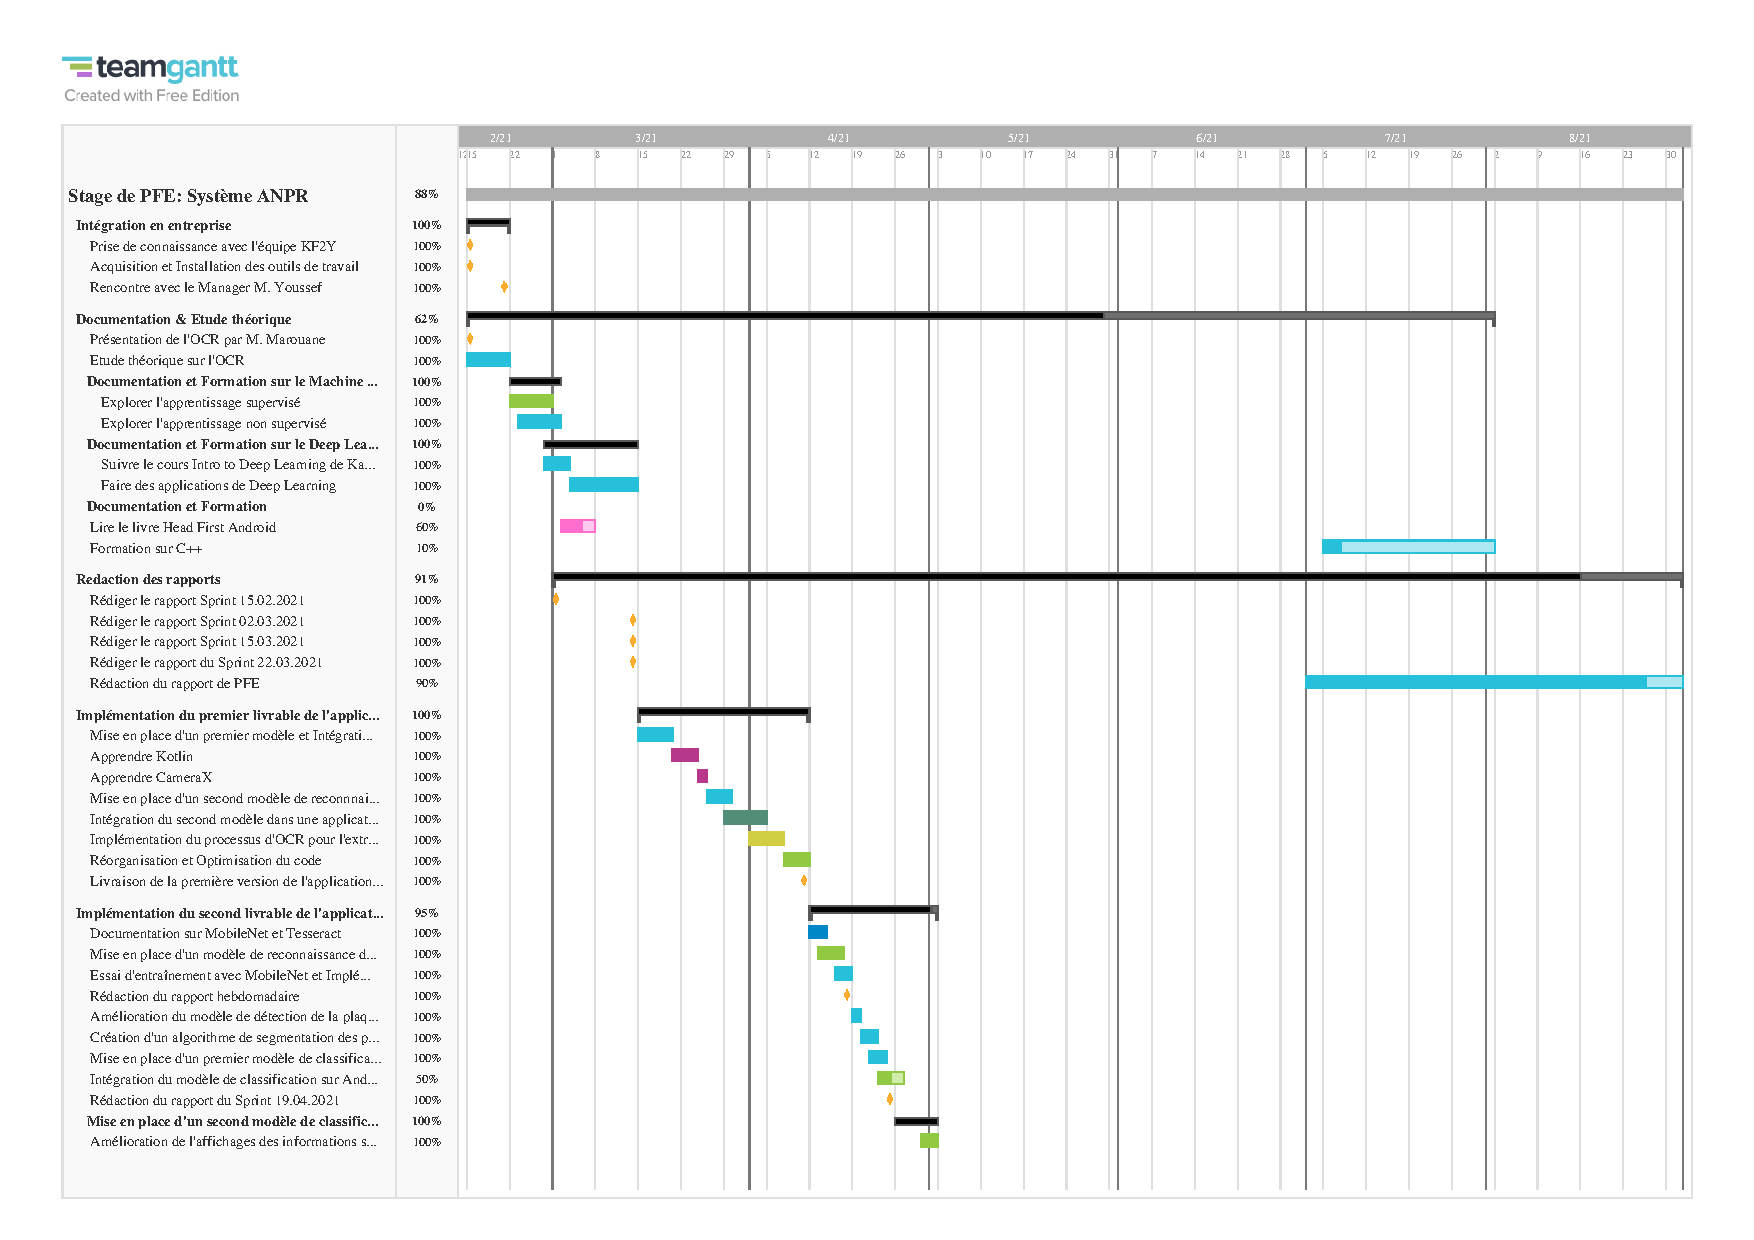
\includegraphics[page=1,width=500pt]{diagrammeGantt.pdf}
    \newpage
    \includegraphics[page=2,width=500pt]{diagrammeGantt.pdf}
\section{Tableau des sprints sur Trello}
    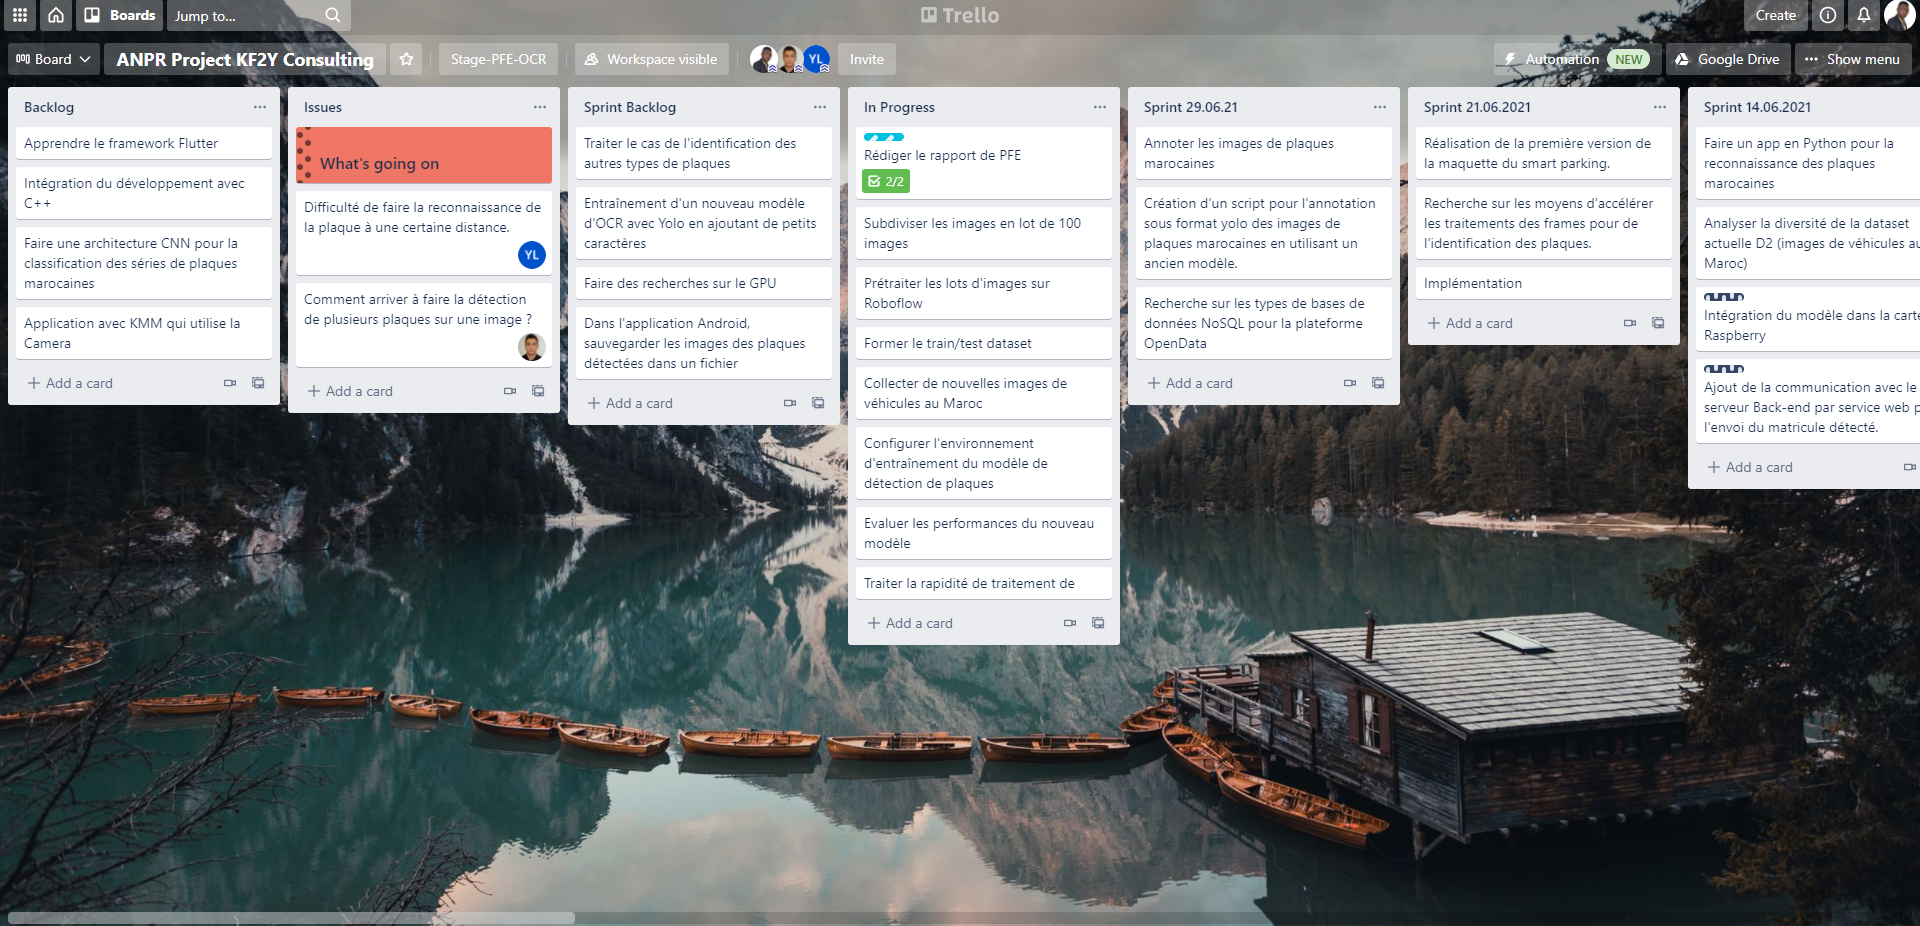
\includegraphics[width=500pt]{tableauTrello.png}

\section{Diagramme UML de l'application mobile}
    \begin{figure}[H]
        \centering
        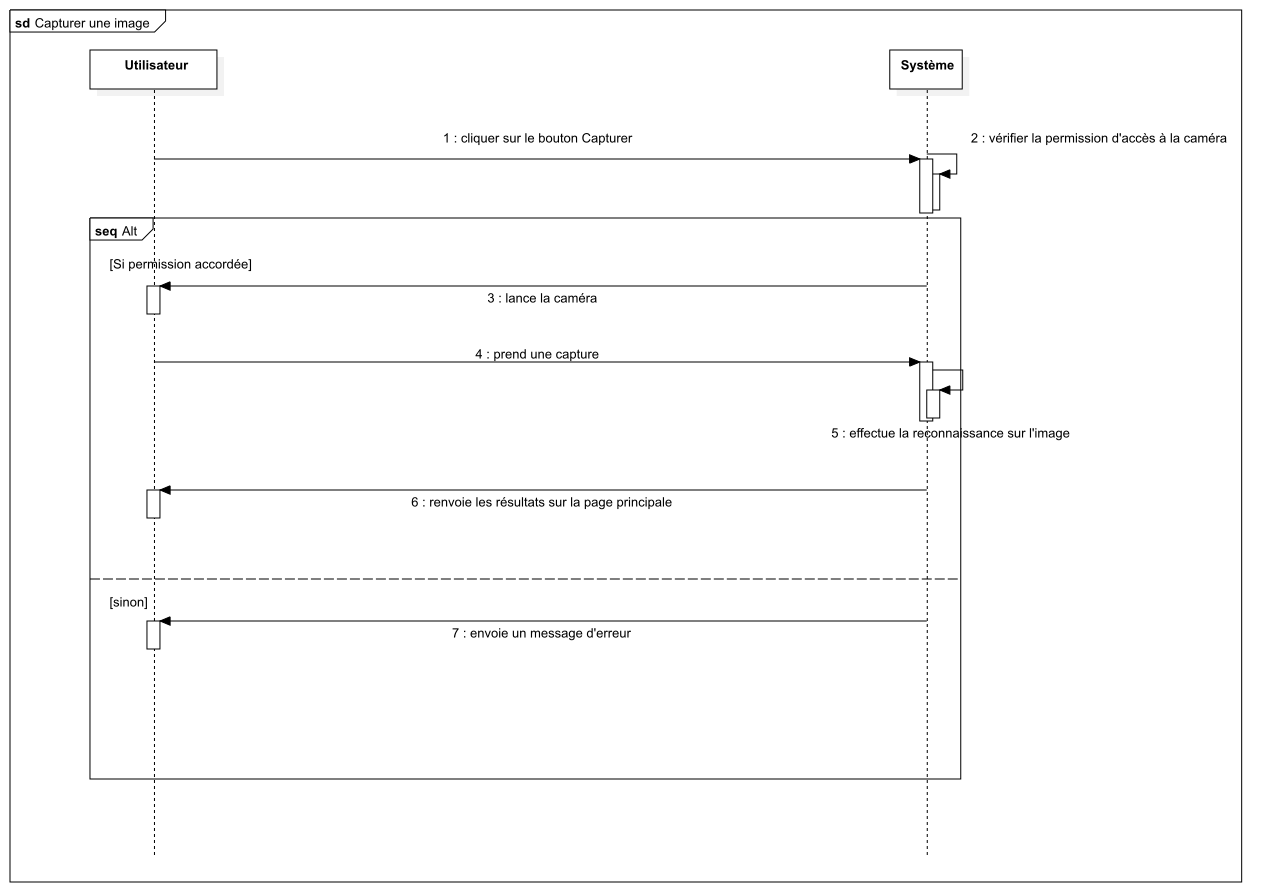
\includegraphics[width=500pt]{sequenceDiagram}
        \caption{Diagramme de séquence pour le cas d'utilisation "Capturer une image"}
        \label{fig:ds1}
    \end{figure}
    \begin{figure}[H]
        \centering
        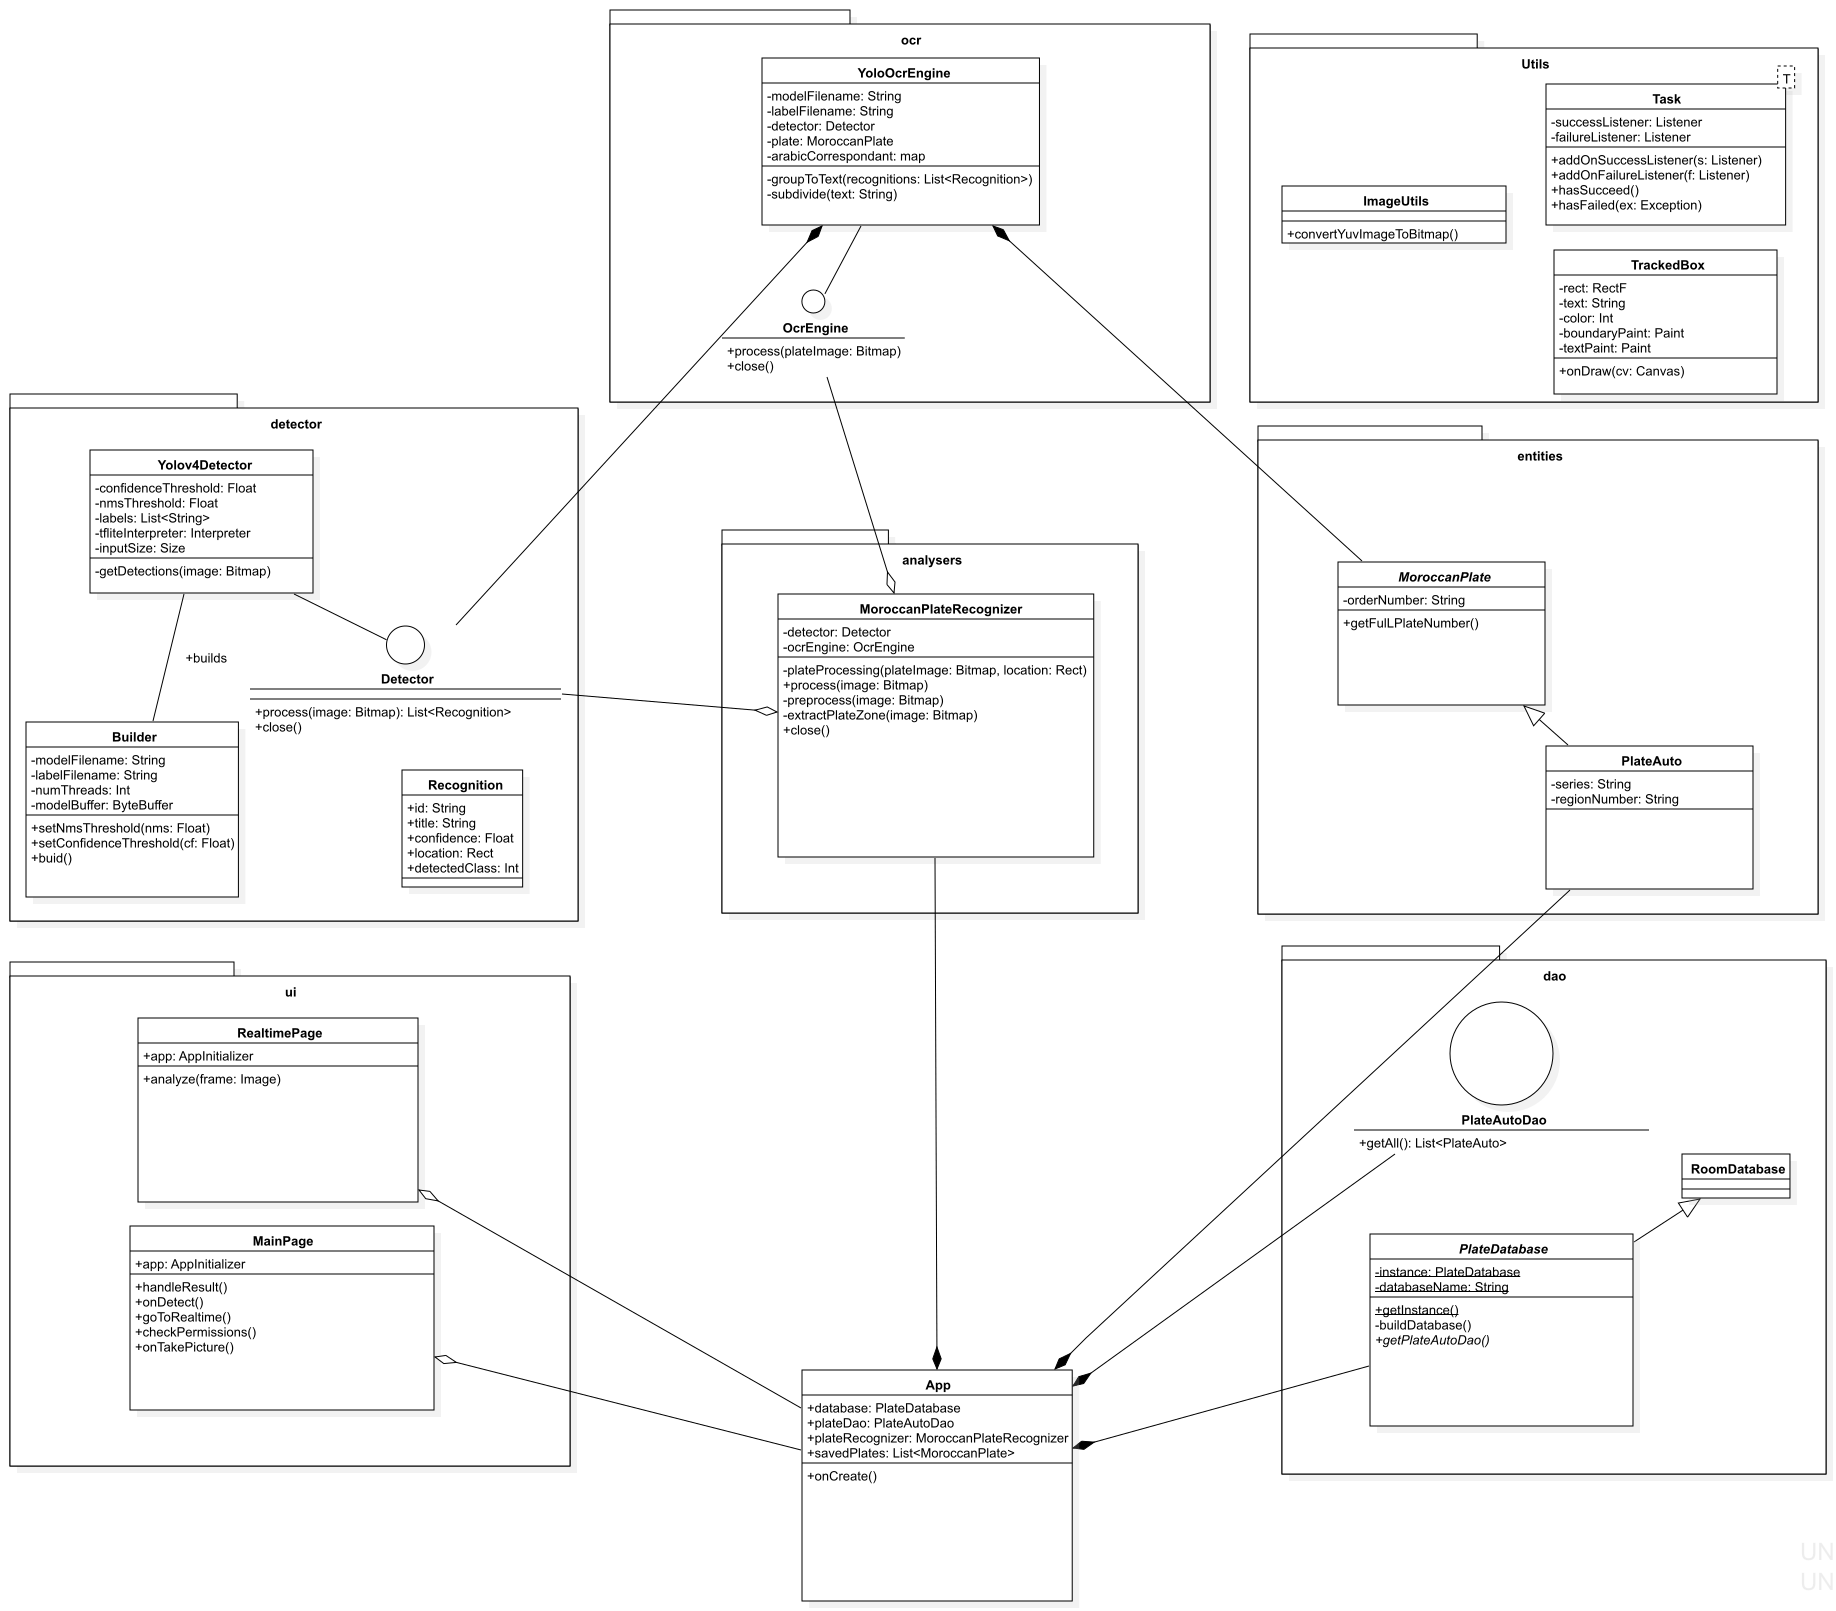
\includegraphics[width=500pt]{ClassDiagram1.png}
        \caption{Architecture détaillée de notre application}
        \label{fig:dc1}
    \end{figure}
    \begin{figure}[H]
        \centering
        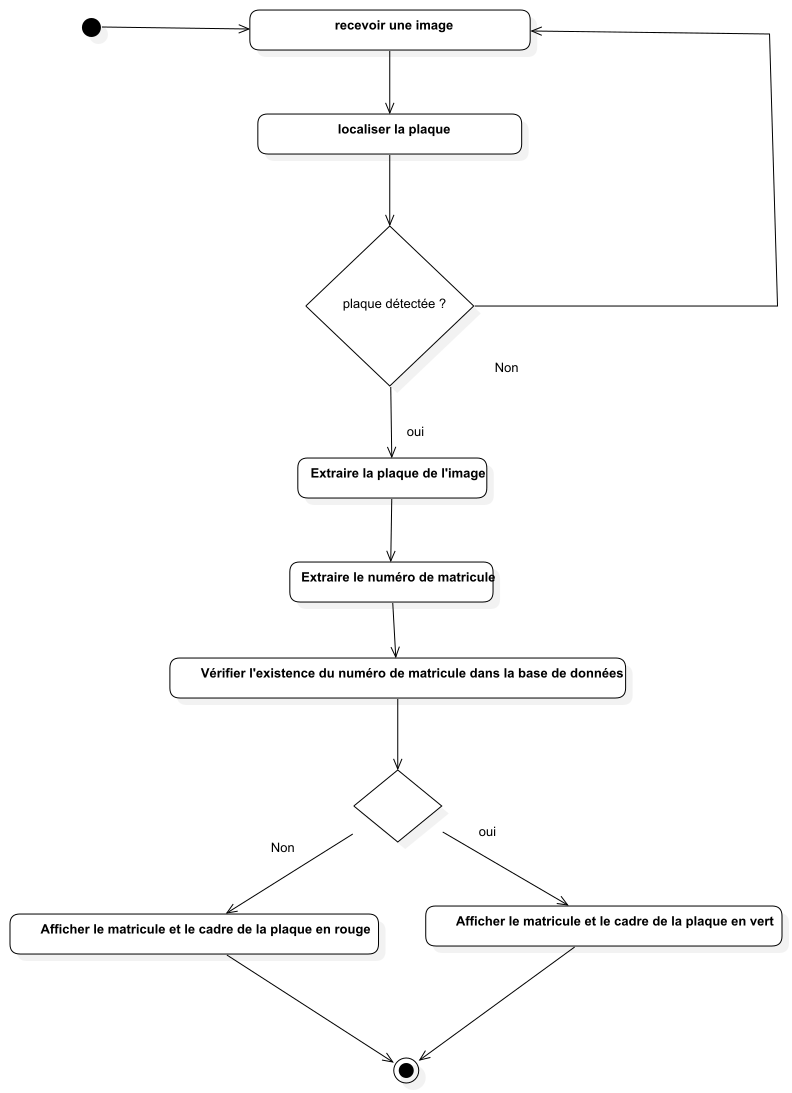
\includegraphics[scale=0.3]{activityDiagram.png}
        \caption{Diagramme d'activité pour la reconnaissance des plaques}
        \label{fig:da1}
    \end{figure}

\section{Architecture d'Android}
\begin{figure}[H]
    \centering
    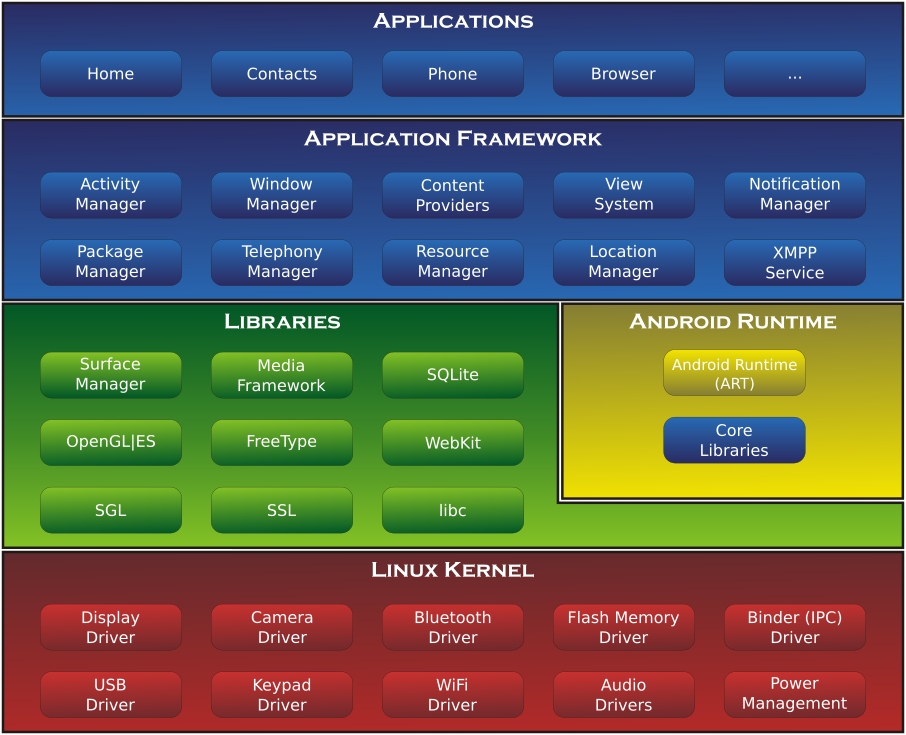
\includegraphics[scale=0.5]{Android-System-Architecture.png}
    \caption{Architecture d'Android}
\end{figure}

\section{Architecture de la bibliothèque Room}
\begin{figure}[H]
    \centering
    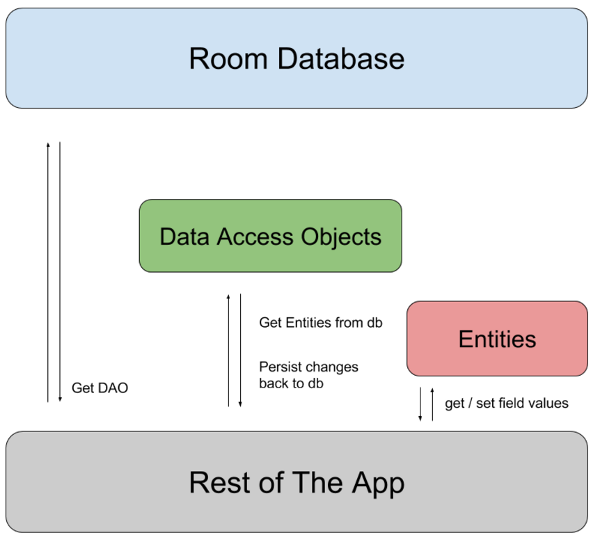
\includegraphics[scale=0.5]{roomArchitecture.png}
    \caption{Architecture de la bibliothèque Room}
    \label{fig:room}
\end{figure}
    
\section{Maquette du parking intelligent}
    \begin{figure}[H]
        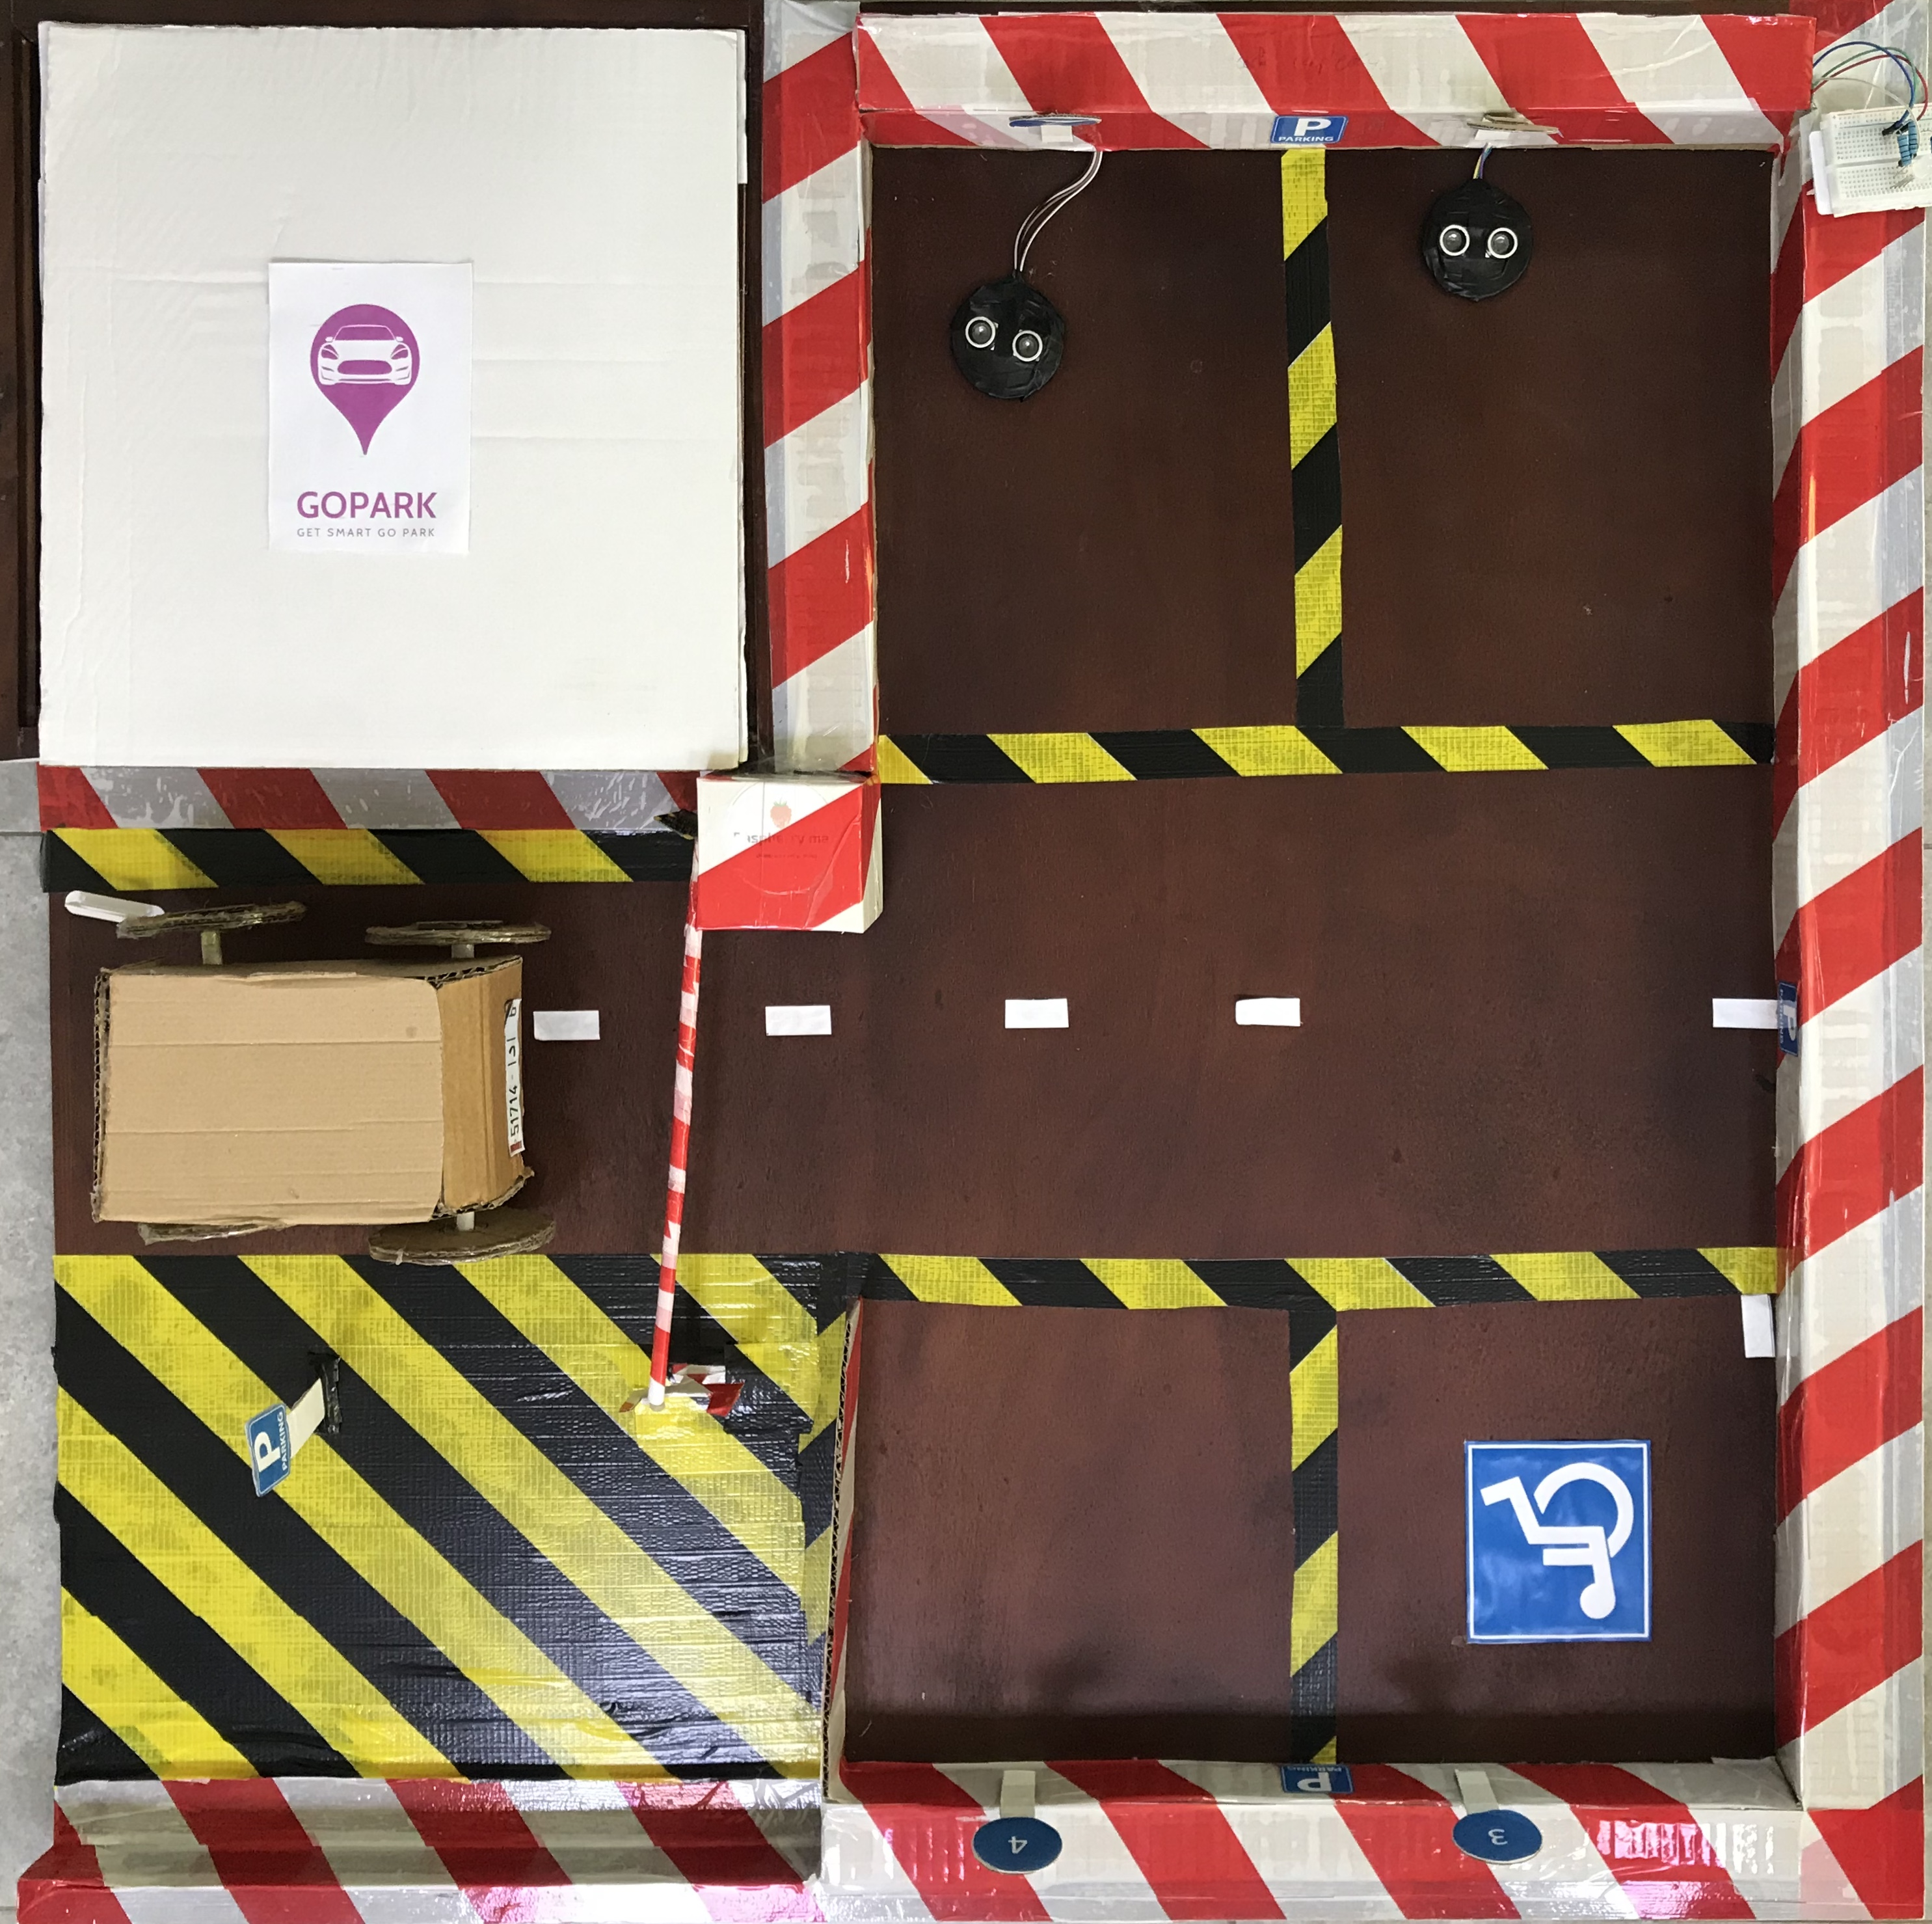
\includegraphics[width=500pt]{maquette}
        \caption{Maquette du parking intelligent}
        \label{fig:maquette}
    \end{figure}

    
\end{document}
